%% ============================================================
%% IEEE MLSP conference paper -- Overleaf-compatible.
%% Compile: pdflatex -> bibtex -> pdflatex -> pdflatex
%% Target: exactly 6 pages, exactly 45 cited references.
%% ============================================================
\documentclass[conference]{IEEEtran}
\usepackage{cite}          % auto-sorts/compresses citation groups
\usepackage{amsmath,amssymb}
\usepackage{graphicx}
\usepackage{booktabs}
\usepackage{multirow}
\usepackage{array}
\usepackage{xcolor}
\usepackage{tikz}
\usetikzlibrary{arrows.meta,positioning,fit,backgrounds,calc}
\usepackage{url}
\usepackage{balance}

\graphicspath{{figures/}}

% compact notation
\newcommand{\dom}{\ensuremath{\mathcal{D}}}
\newcommand{\gain}{\ensuremath{\mathcal{G}}}
\newcommand{\rhof}{\ensuremath{\rho_{\mathrm{fus}}}}
\newcommand{\rhoe}{\ensuremath{\rho_{\mathrm{enc}}}}
\newcommand{\updr}{\ensuremath{r_{\Delta\theta}}}
\newcommand{\gradr}{\ensuremath{r_{g}}}

\begin{document}

\title{Forward or Gradient? Disentangling\\ Training-Time Feature-Scale Effects on Modality Contribution}

\author{\IEEEauthorblockN{Ankita Maji}
\IEEEauthorblockA{Dept. of CSE\\
LPU, Phagwara, India\\
\texttt{ankitamaji7033@gmail.com}}
\and
\IEEEauthorblockN{Koman Lamba}
\IEEEauthorblockA{Dept. of CSE\\
LPU, Phagwara, India\\
\texttt{ankitamaji7033@gmail.com}}
\and
\IEEEauthorblockN{Prabhutee}
\IEEEauthorblockA{Dept. of CSE\\
LPU, Phagwara, India\\
\texttt{ankitamaji7033@gmail.com}}}

\maketitle

\begin{abstract}
Multimodal networks frequently under-use one modality, and feature-magnitude imbalance is often invoked as an explanation. We ask a sharper, mechanistic question: how does a \emph{training-time}, modality-specific feature-scale intervention alter learned modality contribution, and through which pathway---the forward representation magnitude, the encoder-gradient magnitude, or both? Using custom autograd operators that rescale one modality's fused representation in the forward pass only, the backward pass only, or both while leaving the training objective unchanged, we separate the two pathways and record the encoder parameter-update ratio as an optimization-level readout. Across a synthetic generator and two real datasets (CREMA-D, UTD-MHAD): a constant scale is largely compensated by trainable encoders; the training-time intervention nonetheless produces substantial changes in contribution; under the tested Adam configuration forward scaling carries the effect while isolated gradient scaling changes little despite $100$--$282\times$ gradient-norm ratios (update ratio $\approx\!1$); under SGD both pathways contribute (gradient-only update ratio $\approx\!96\times$ at $\alpha{=}100$). On CREMA-D, forward scaling closely matches the effect ($d\!\approx\!7.4$) and gradient scaling does not. As boundary conditions, the forward effect varies across the evaluated fusion mechanisms (attenuated under gated fusion) while gradient-only stays approximately null, and in a utility-asymmetric setting (UTD-MHAD) the response to scaling differs sharply with modality utility. Normalization suppresses the imposed-scale difference but is not a cure.
\end{abstract}

\begin{IEEEkeywords}
Multimodal learning, modality imbalance, feature scaling, gradient dynamics, optimization, fusion, controlled interventions.
\end{IEEEkeywords}

\section{Introduction}
Combining complementary signals such as audio and video, or depth and inertial motion, is central to multimodal signal processing~\cite{ramachandram2017deep,baltrusaitis2019multimodal,atrey2010multimodal}. Yet jointly trained multimodal classifiers routinely under-exploit one modality, converging to a solution dominated by the other even when both carry task-relevant information~\cite{wang2020what,peng2022balanced,huang2022modality}. Because encoders emit representations at different magnitudes, a common intuition is that feature-scale imbalance down-weights the weaker branch. This motivates normalization and rebalancing methods, but is rarely tested by intervention: correlational evidence cannot separate whether scale acts through the \emph{forward} representation or the \emph{backward} gradient that updates each encoder.

We treat $\alpha$ as an externally controlled intervention rather than an observed correlate~\cite{pearl2009causality}, and study a single, well-defined manipulation: multiplying one modality's fused representation by a constant $\alpha$ at the fusion boundary while both encoders remain trainable. The central question is whether a training-time modality-specific feature-scale intervention acts through the forward-representation-magnitude pathway, the encoder-gradient pathway, or both, and how this depends on optimizer, fusion mechanism, and modality utility.

To answer it we introduce a controlled autograd intervention that separates the forward-representation and backward-gradient consequences of the scaling under a fixed objective, and record the encoder parameter-update ratio as an optimization-level readout. Our contribution is methodological rather than another rebalancing algorithm; concretely:
\begin{itemize}
\item A controlled forward-only/gradient-only/ordinary intervention that isolates the two pathways of a training-time feature-scale change under a fixed objective (Section~\ref{sec:formulation}).
\item A mechanistic finding that the pathway carrying the effect is optimizer-dependent---forward-associated under Adam (isolated gradient scaling produces little change) and forward-plus-gradient under SGD---tracked by the parameter-update ratio (Section~\ref{sec:synthetic}).
\item Real-data corroboration on CREMA-D and boundary analyses: fusion mechanism (sum/concat/gated), UTD-MHAD utility asymmetry, and normalization (Section~\ref{sec:real},~\ref{sec:boundary}).
\end{itemize}

\section{Related Work}
\textbf{Multimodal fusion.} Fusion ranges from early/late strategies~\cite{snoek2005early,ngiam2011multimodal} to tensor and attention mechanisms~\cite{zadeh2017tensor,nagrani2021attention}, with broad surveys of design choices~\cite{baltrusaitis2019multimodal,liang2024foundations}; multimodal training can under-perform the best unimodal model, motivating analyses of when fusion helps~\cite{wang2020what,huang2021what}.

\textbf{Modality imbalance and rebalancing.} One modality often dominates optimization: greedy learning dynamics~\cite{wu2022characterizing}, modality competition~\cite{huang2022modality}, and uni-modal feature under-learning~\cite{du2023unimodal}. Remedies modulate the learning signal---on-the-fly gradient modulation (OGM-GE)~\cite{peng2022balanced}, adaptive gradient modulation~\cite{li2023boosting}, prototypical rebalancing~\cite{fan2023pmr}, alternating unimodal adaptation~\cite{zhang2024mla}, per-modality learning-rate tracking~\cite{sun2021learning}, functional-entropy regularization~\cite{gat2020removing}, and calibration~\cite{ma2023calibrating}. These act on \emph{which loss or gradient trains the encoder}; unlike such rebalancing methods, our intervention is designed as a diagnostic---the objective is held fixed while the forward and backward consequences of the same scale perturbation are independently controlled to identify which pathway carries the effect.

\textbf{Gradient balancing in multi-task learning} adjusts per-task gradients by norm or direction~\cite{chen2018gradnorm,yu2020gradient,kendall2018multi}; these differ from our single-intervention pathway separation under one fixed objective.

\textbf{Optimization.} Whether a per-modality gradient rescale changes learning depends on the optimizer. Adam's~\cite{kingma2015adam} coordinate-wise second-moment normalization can attenuate a \emph{constant} gradient rescale, studied through the sign/variance structure of adaptive updates~\cite{balles2018dissecting,bernstein2018signsgd,kunstner2023noise} and connected to why adaptive methods differ from SGD~\cite{wilson2017marginal,zhang2020why,reddi2018convergence,loshchilov2019decoupled}; SGD with momentum~\cite{sutskever2013importance} instead passes gradient scale into the update. We use this optimizer literature to interpret---not to claim---our findings: the optimizer-level attenuation itself is not presented as new; our contribution is connecting it, via matched pathway interventions, to modality-contribution changes under training-time feature scaling.

\textbf{Normalization.} Batch, layer, and group normalization~\cite{ioffe2015batch,ba2016layer,wu2018group} and analyses of their optimization effects~\cite{santurkar2018how} remove magnitude differences; we use per-modality standardization as a control on the imposed scale channel, not a cure. Quantifying each modality's contribution is itself subtle~\cite{hessel2020does}; we adopt an interventional stance~\cite{pearl2009causality} on standard audio-visual and multimodal-sensing benchmarks~\cite{cao2014crema,chen2015utd,arandjelovic2017look,owens2018audio,ephrat2018looking}.

\section{Problem Formulation and Controlled Interventions}
\label{sec:formulation}
\subsection{Modality-Specific Feature-Scale Intervention}
Let $h_A,h_B$ be the modality representations entering fusion $f(\cdot)$ with a classifier head trained by cross-entropy. The intervention multiplies one branch (say $A$) by a constant $\alpha$ at the fusion boundary, $h_A \leftarrow \alpha\, h_A$, with both encoders trainable throughout. This is a training-time, not test-time, manipulation: the scaled representation shapes fusion, loss, and gradients at every step. Following an interventional view~\cite{pearl2009causality}, $\alpha$ is set exogenously, so contrasts across $\alpha$ quantify the response to the imposed scale intervention rather than an observational association with naturally occurring feature magnitude. We use intervention terminology to distinguish exogenously assigned perturbations from observational correlations; we do not claim identification of a complete causal graph.

\subsection{Forward and Gradient Pathways}
Let $\tilde h_A$ be the representation that enters fusion. For the ordinary multiply $\tilde h_A=\alpha h_A$, the chain rule couples two effects at once: the forward activation is enlarged, and $\partial L/\partial h_A=\alpha\,\partial L/\partial\tilde h_A$, so the gradient (and hence the update) to encoder $A$ also carries $\alpha$. To disentangle them we define two custom autograd operators with independent forward and backward maps:
\begin{align}
\textsc{Fwd}_\alpha:&\quad \tilde h_A=\alpha h_A,\ \ \tfrac{\partial L}{\partial h_A}=\tfrac{\partial L}{\partial \tilde h_A}\ (\times 1),\\
\textsc{Grad}_\alpha:&\quad \tilde h_A=h_A,\ \ \ \tfrac{\partial L}{\partial h_A}=\alpha\,\tfrac{\partial L}{\partial \tilde h_A}\ (\times \alpha).
\end{align}
Four arms then share one objective: \emph{baseline} ($\tilde h_A=h_A$), \emph{forward-only} ($\textsc{Fwd}_\alpha$: forward scaled, gradient unscaled), \emph{gradient-only} ($\textsc{Grad}_\alpha$: forward unchanged, gradient scaled), and \emph{ordinary} ($\alpha h_A$: both), so ordinary is the composition of the two isolated maps. The operator acts at the fusion boundary---after each encoder (and its normalization), before fusion---on modality $A$ only; in the gradient-only arm the forward pass, loss, and classifier-head gradients are therefore unchanged by construction ($\textsc{Grad}_\alpha$ is the identity in the forward pass), and only modality $A$'s encoder gradient is multiplied by $\alpha$, entering the optimizer as a constant per-parameter rescale (no weight decay, gradient clipping, or scheduler is used). A sanity gate verifies each operator's forward/backward multipliers (baseline $1{,}1$; forward $\alpha{,}1$; gradient $1{,}\alpha$; ordinary $\alpha{,}\alpha$) before training; runs that diverge are recorded and excluded (none did).

\subsection{Modality Contribution Metrics}
We use \emph{masked} unimodal accuracy as an operational contribution measure: $\mathrm{Acc}_A$ is the joint model's accuracy when modality $B$'s fused input is zeroed (and vice versa). Because masking is not necessarily part of the training distribution, it is a diagnostic of retained modality-specific predictive utility, not a calibrated estimate of causal contribution. From it we report dominance $\dom=\mathrm{Acc}_A-\mathrm{Acc}_B$ and multimodal gain $\gain=\mathrm{Acc}_{AB}-\max(\mathrm{Acc}_A,\mathrm{Acc}_B)$, with $\mathrm{Acc}_{AB}$ the joint accuracy. As magnitude readouts we use the fusion-input norm ratio $\rhof=\lVert h_A\rVert/\lVert h_B\rVert$ (post-scale) and the pre-scale ratio $\rhoe$ (compensation), and we record the encoder parameter-update ratio $\updr=\lVert\Delta\theta_A\rVert/\lVert\Delta\theta_B\rVert$ alongside the gradient-norm ratio $\gradr$. Because $\updr$ is what changes weights, we use it as an optimization-level readout of how a gradient rescale becomes an update, not a formal mediation analysis.

\subsection{Experimental Hypotheses}
Within the defined experimental regimes we test: (H1) a constant modality-specific scale held fixed throughout training (encoders trainable) is substantially compensated, leaving only a small residual contribution change; (H2) the training-time forward-scale intervention changes learned contribution; (H3) under the tested Adam configuration isolated gradient scaling produces a substantially weaker effect than forward scaling; (H4) under SGD, gradient/update scaling contributes more strongly to the observed effect; (H5) the observed forward effect varies across the evaluated fusion mechanisms and differs qualitatively between the matched synthetic setting and the utility-asymmetric real-data setting tested.

\begin{figure}[t]
\centering
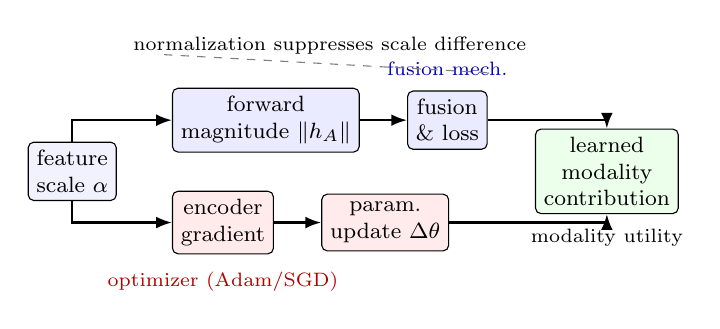
\begin{tikzpicture}[
  font=\footnotesize,
  box/.style={draw,rounded corners=2pt,align=center,inner sep=3pt,minimum height=6.5mm,fill=blue!5},
  fwdbox/.style={box,fill=blue!8},
  grdbox/.style={box,fill=red!8},
  arr/.style={-{Latex[length=2mm]},thick},
  >=Latex]
\node[box] (scale) {feature\\scale $\alpha$};
\node[fwdbox,right=7mm of scale,yshift=6.5mm] (fwd) {forward\\magnitude $\lVert h_A\rVert$};
\node[grdbox,right=7mm of scale,yshift=-6.5mm] (grd) {encoder\\gradient};
\node[fwdbox,right=6mm of fwd] (fus) {fusion\\ \& loss};
\node[grdbox,right=6mm of grd] (upd) {param.\\update $\Delta\theta$};
\node[box,right=6mm of fus,yshift=-6.5mm,fill=green!8,minimum height=9mm] (con) {learned\\modality\\contribution};
\draw[arr] (scale) |- (fwd);
\draw[arr] (scale) |- (grd);
\draw[arr] (fwd) -- (fus);
\draw[arr] (grd) -- (upd);
\draw[arr] (fus) -| (con);
\draw[arr] (upd) -| (con);
\node[below=1.0mm of grd,red!70!black,font=\scriptsize] {optimizer (Adam/SGD)};
\node[above=0.6mm of fus,blue!70!black,font=\scriptsize] {fusion mech.};
\node[below=0.6mm of con,font=\scriptsize] {modality utility};
\draw[dashed,gray] ($(fwd.north west)+(-1mm,4.2mm)$) -- ($(fus.north east)+(1mm,2.2mm)$)
   node[midway,above,font=\scriptsize,black] {normalization suppresses scale difference};
\end{tikzpicture}
\caption{Conceptual decomposition of the training-time scale intervention (not an identified causal graph). A modality-specific scale factor can act through a forward-magnitude pathway (into fusion and loss) and a backward pathway (into the parameter update). Optimizer, fusion mechanism, and modality utility moderate the effect; per-modality normalization largely suppresses the imposed forward-scale difference.}
\label{fig:causal}
\end{figure}

\section{Controlled Synthetic Study}
\label{sec:synthetic}
\subsection{Experimental Setup}
Each modality is generated by $x_m=\alpha_m(\mu^m_y+\sigma_m\varepsilon)$, $\varepsilon\!\sim\!\mathcal{N}(0,I)$, with orthonormal class prototypes $\mu^m$ of norm (separation scale) $1.5$ drawn from a fixed seed, $C{=}8$ classes, $d_a{=}d_v{=}32$, $\sigma{=}1$, and $4000/1000/2000$ samples. Because a linear head can in principle absorb a constant $\alpha_m$, a fixed feature rescaling need not remove the information available to the classifier; both modalities share prototype geometry and noise variance (matched generative signal-to-noise). Encoders are matched two-layer MLPs (hidden $64$, ReLU, rep dim $32$), sum fusion (unless stated), linear head, Adam, batch $256$, $40$ epochs, five seeds on the fixed split (Table~\ref{tab:protocol}); PyTorch~\cite{paszke2019pytorch}. Throughout, significance is a two-sided paired $t$-test across the five seeds and Cohen's $d_z$ is the paired mean difference over its standard deviation---the identical routine for every comparison, pre-specified and without multiplicity correction. With $n{=}5$ on a \emph{fixed} split, effect sizes and $p$-values quantify within-split reproducibility, not population inference; a large $|d|$ reflects cross-seed consistency, not a large population effect. Zero of $60$ (disentanglement) and $60$ (fusion) runs diverged.

\subsection{A Constant Scale Is Compensated}
We first ask whether a \emph{constant} modality-specific scale---held fixed throughout training with both encoders trainable (not an inference-time rescale of a frozen encoder)---is by itself a persistent cause. The encoders adapt: as the imposed scale grows, $\rhoe$ moves oppositely and contribution returns toward baseline, so under the evaluated synthetic regime a constant scale is substantially compensated, leaving only a small residual contribution change over the tested range (H1).

\subsection{Scale $\times$ Optimization Interaction}
These controlled interventions provide a setting for distinguishing the forward-scale and optimization pathways; we summarize persistence by a study-specific statistic $S_{\mathrm{loss}}=\mathrm{clip}(1-c_{\mathrm{weak}}/c_{\mathrm{weak}}^{\mathrm{base}},0,1)$ (fractional reduction of the weak modality's contribution below its balanced baseline), not proposed as a universal definition of modality collapse. A constant feature-scale imbalance stays compensable ($S_{\mathrm{loss}}$ remains $0.04$--$0.08$ across $20$--$400\times$), whereas a learning-rate imbalance, or a scale-and-LR-aligned imbalance, produces persistent contribution loss ($S_{\mathrm{loss}}\!\to\!0.88$ and $1.0$ at $400\times$)---here associated more with the optimization/learning-rate channel than with feature scale alone.

\subsection{Forward-vs-Gradient Disentanglement}
Under Adam~\cite{kingma2015adam} at $\alpha\!=\!100$ (Fig.~\ref{fig:disentangle}a, Table~\ref{tab:disentangle}), forward-only shifts dominance ($\Delta\dom\!=\!-0.070$, $d\!=\!-3.76$, $p\!=\!1.1\!\times\!10^{-3}$) and closely matches the ordinary intervention ($\Delta\dom\!=\!-0.069$; ordinary$\approx$forward). Gradient-only produces little change ($\Delta\dom\!=\!-5\!\times\!10^{-4}$, $d\!=\!-0.53$, $p\!=\!0.30$) even though it inflates the gradient-norm ratio by more than two orders of magnitude. The update readout tracks this (Fig.~\ref{fig:disentangle}b): under Adam the gradient-only arm leaves the parameter-update ratio at $\updr\!\approx\!1$, consistent with the attenuation expected from Adam's normalized update under approximately constant gradient rescaling~\cite{balles2018dissecting,bernstein2018signsgd,kunstner2023noise}.

\subsection{Optimizer Dependence}
Repeating the decomposition under SGD with momentum $0.9$~\cite{sutskever2013importance} (same lr $10^{-3}$, $40$ epochs) changes the picture (Table~\ref{tab:disentangle}). Now gradient-only \emph{does} shift dominance ($\Delta\dom\!=\!+0.200$, $d\!=\!3.90$) with an $\approx\!96\times$ update ratio ($\updr\!=\!95.9$ at $\alpha{=}100$): the gradient scale is substantially transmitted into the parameter update, behaving like a substantial effective per-modality learning-rate difference in this setting. Forward-only also acts ($\Delta\dom\!=\!+0.244$, $d\!=\!3.93$), and ordinary ($\Delta\dom\!=\!+0.322$) exceeds forward ($d_{\text{ord vs fwd}}\!=\!2.86$, $p\!=\!3\!\times\!10^{-3}$). Both pathways contribute; the ordinary shift is smaller than the sum of the isolated forward and gradient shifts ($0.322<0.244+0.200$), i.e.\ the two effects do not combine additively here. Within the tested configurations, optimizer behavior determines which pathway more strongly transmits the intervention (H3--H4).

\begin{figure*}[t]
\centering
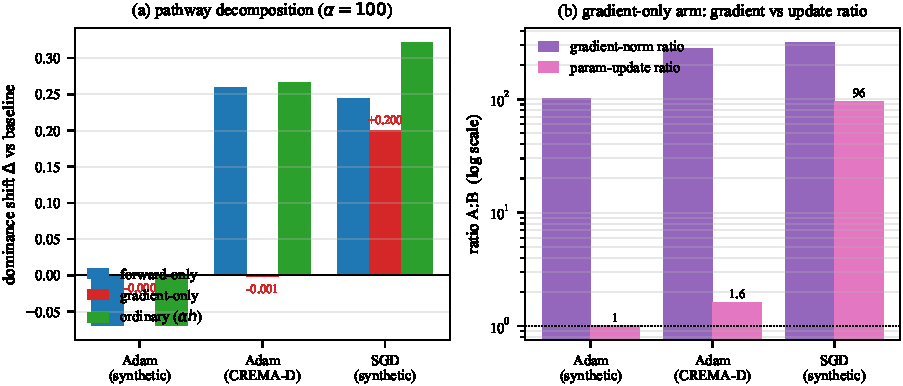
\includegraphics[width=0.62\textwidth]{fig_disentangle.pdf}
\caption{Forward-vs-gradient decomposition at $\alpha\!=\!100$ (five seeds). (a) Signed dominance shift by arm; the gradient-only bar is $\approx\!0$ under Adam (synthetic, CREMA-D) but large under SGD, forward-only tracks ordinary. (b) Gradient-only arm, gradient-norm vs update ratio (log): under Adam a $100$--$283\times$ gradient ratio gives an update ratio $\approx\!1$; under SGD $\approx\!96\times$.}
\label{fig:disentangle}
\end{figure*}

\section{Real-Data Evidence}
\label{sec:real}
\subsection{CREMA-D Setup}
CREMA-D~\cite{cao2014crema} provides audio-video emotional utterances over six classes. We use an actor-disjoint split ($64/9/18$ actors $=5234/738/1470$ clips), reducing the possibility that the reported effect is driven by actor overlap between splits. Audio is $16$\,kHz mono, $3$\,s, encoded as a $64$-bin log-mel spectrogram; video is $8$ uniformly sampled $64\times64$ grayscale frames. Both encoders are matched three-block CNNs~\cite{he2016deep} (Table~\ref{tab:protocol}) producing $64$-d representations combined by sum fusion with a linear head; audio is the scaled modality, $\alpha\!\in\!\{10,100\}$. The baseline is genuinely multimodal (Table~\ref{tab:cremad}; joint accuracy $0.493$, gain $0.248$, dominance $0.075$).

\subsection{Training-Time Scaling Results}
Scaling one modality during training monotonically reshapes contribution (Table~\ref{tab:cremad}): amplifying audio raises audio dominance ($0.075\!\to\!0.299\!\to\!0.328$ at $1/5/10\times$) and reduces multimodal gain from $0.248$ to $0.013$, while amplifying video does the opposite (dominance $\to\!0.009$, gain $\to\!0.295$); imposed scale and learned dominance are rank-correlated (Spearman $0.922$). The pre-scale ratio $\rhoe$ shifts oppositely, consistent with partial encoder compensation; per-modality $z$-scoring largely suppresses the imposed difference (audio-$10\times$: dominance $0.328\!\to\!0.110$, $\rhof\;3.24\!\to\!0.97$; Table~\ref{tab:cremad}), analyzed in \S\ref{sec:boundary}.

\subsection{Real-Data Forward-vs-Gradient Disentanglement}
The same four-arm decomposition on CREMA-D ($40$ runs, $0$ diverged) matches the Adam pattern (Fig.~\ref{fig:disentangle}, Table~\ref{tab:disentangle}). Forward-only produces the effect ($\Delta\dom\!=\!+0.259$, $d\!=\!7.39$, $p\!=\!8\!\times\!10^{-5}$) and closely matches ordinary ($d_{\text{ord vs fwd}}\!=\!0.59$, $p\!=\!0.26$). Gradient-only produced no detectable shift (five seeds; $\Delta\dom\!=\!-0.001$, $d\!=\!-0.08$, $p\!=\!0.87$) despite a $282\times$ gradient-norm ratio, its update ratio being only $1.61$.

\section{Fusion and Modality-Utility Boundaries}
\label{sec:boundary}
\subsection{Fusion-Mechanism Robustness}
We repeat the decomposition under three fusion mechanisms---sum, concatenation, and learned gated fusion (per-modality sigmoid self-gates)---over $60$ runs, $0$ diverged (Fig.~\ref{fig:fusion}). Across all three evaluated mechanisms, gradient-only produced little measurable contribution shift ($|\Delta\dom|\!\le\!0.001$, update ratio $\approx\!1$). The observed forward effect, however, varied across the evaluated fusion mechanisms: strong under sum ($d\!=\!-3.76$, $p\!=\!1\!\times\!10^{-3}$) and concatenation ($d\!=\!-5.16$, $p\!=\!3\!\times\!10^{-4}$), but attenuated under gated fusion ($d\!=\!-0.70$), where it was \emph{not} individually significant ($p\!=\!0.19$), consistent with the possibility that the learned per-modality gates can partly absorb the imposed forward magnitude---variation across the evaluated mechanisms, not architecture generality.

\subsection{UTD-MHAD: A Modality-Utility Boundary}
UTD-MHAD~\cite{chen2015utd} pairs depth and inertial sensing over $27$ actions ($861$ usable samples), subject-disjoint split (Table~\ref{tab:protocol}). The modalities exhibit strongly asymmetric predictive utility: masked depth accuracy is near the $27$-class chance level ($0.037$), at $0.036$ (so the dominance metric is influenced by the large difference in unimodal predictive utility), while inertial is informative ($0.227$), with strong multimodal accuracy ($0.632$, gain $0.405$). We therefore include UTD as a boundary-condition experiment---a utility-asymmetry test, \emph{not} an independent replication of the central pathway decomposition (Fig.~\ref{fig:utd}). The response to scaling differed sharply: amplifying the informative inertial modality further increased its relative contribution (dominance $-0.191\!\to\!-0.615$, gain $\to\!0.053$), whereas amplifying the near-chance depth modality barely moved contribution (dominance $\to\!-0.198$, gain $\approx\!0.40$). Because the test set is four fixed subjects, we report per-subject consistency and do not treat seed-level $p$-values as population inference.

\subsection{Normalization Analysis}
Per-modality standardization largely suppresses the imposed forward-scale difference ($\rhof\!\to\!\approx\!1$) and substantially reduces the induced contribution shift, but does not improve (and can slightly reduce) accuracy and does not directly modify the optimization imbalance seen in the scale$\times$LR experiments---a control on the imposed scale difference, not a general cure.

\begin{table}[t]
\caption{Forward-vs-gradient decomposition ($\alpha\!=\!100$, five seeds). $\Delta\dom$: dominance shift vs baseline; $\gradr,\updr$: gradient-norm and parameter-update ratios for the stated arm.}
\label{tab:disentangle}
\centering
\footnotesize
\begin{tabular}{@{}llrrr@{}}
\toprule
Setting & Arm & $\Delta\dom$ & Cohen's $d$ & $p$ \\
\midrule
\multirow{3}{*}{Adam, synthetic} & forward  & $-0.070$ & $-3.76$ & $1.1\!\times\!10^{-3}$ \\
                                 & gradient & $-0.0005$ & $-0.53$ & $0.30$ \\
                                 & ordinary & $-0.069$ & $-3.73$ & $1.1\!\times\!10^{-3}$ \\
\midrule
\multirow{3}{*}{Adam, CREMA-D}   & forward  & $+0.259$ & $+7.39$ & $8\!\times\!10^{-5}$ \\
                                 & gradient & $-0.001$ & $-0.08$ & $0.87$ \\
                                 & ordinary & $+0.266$ & $+8.51$ & $4\!\times\!10^{-5}$ \\
\midrule
\multirow{3}{*}{SGD, synthetic}  & forward  & $+0.244$ & $+3.93$ & $9\!\times\!10^{-4}$ \\
                                 & gradient & $+0.200$ & $+3.90$ & $1\!\times\!10^{-3}$ \\
                                 & ordinary & $+0.322$ & $+7.75$ & $7\!\times\!10^{-5}$ \\
\midrule
\multicolumn{2}{@{}l}{gradient-only $\updr$}: & Adam $1.61$ & \multicolumn{2}{r}{SGD $95.9$}\\
\multicolumn{2}{@{}l}{gradient-only $\gradr$}: & Adam $282.7$ & \multicolumn{2}{r}{SGD $318.5$}\\
\bottomrule
\end{tabular}
\end{table}

\begin{table}[t]
\caption{CREMA-D training-time scale (five seeds, Adam). Dominance $\dom$ (audio$-$video) and gain $\gain$; imposed scale and dominance are rank-correlated (Spearman $0.922$). Last row: per-modality $z$-score on audio-$10\times$.}
\label{tab:cremad}
\centering
\footnotesize
\begin{tabular}{@{}lrrr@{}}
\toprule
Condition & $\dom$ & $\gain$ & $\rhof$ \\
\midrule
baseline ($1\times$)      & $0.075$ & $0.248$ & $1.22$ \\
audio $\times5$           & $0.299$ & $0.045$ & $2.31$ \\
audio $\times10$          & $0.328$ & $0.013$ & $3.24$ \\
video $\times5$           & $0.056$ & $0.263$ & $1.18$ \\
video $\times10$          & $0.009$ & $0.295$ & $1.02$ \\
audio $\times10$ + $z$    & $0.110$ & --      & $0.97$ \\
\bottomrule
\end{tabular}
\end{table}

\begin{figure}[t]
\centering
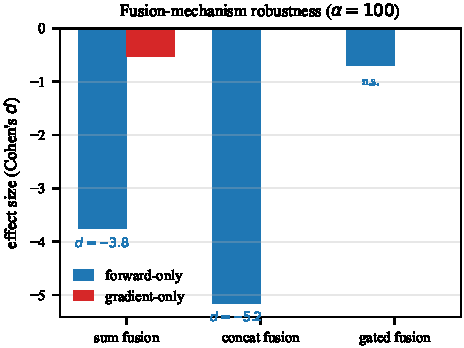
\includegraphics[width=0.66\columnwidth]{fig_fusion.pdf}
\caption{Fusion-mechanism comparison ($\alpha\!=\!100$). Gradient-only is approximately null across all three; the forward effect is strong under sum/concat, attenuated (n.s.) under gated fusion.}
\label{fig:fusion}
\end{figure}

\begin{figure}[t]
\centering
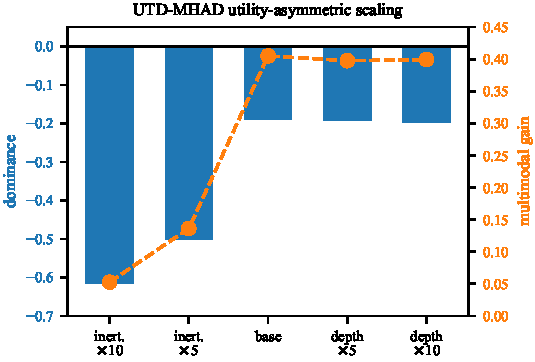
\includegraphics[width=0.66\columnwidth]{fig_utd.pdf}
\caption{UTD-MHAD under modality-utility asymmetry. Amplifying the informative inertial modality further increases its relative contribution and reduces gain; amplifying the near-chance depth modality barely changes contribution.}
\label{fig:utd}
\end{figure}

\begin{table}[t]
\caption{Datasets and protocol (reproducibility). CNN encoders use three conv blocks (conv$\to$ReLU$\to2{\times}2$ max-pool; $2\times$ pooling for the 1D encoder) then global-average pooling and a linear projection to the representation dim: 2D $3{\times}3$ with $16/32/32$ channels (CREMA audio/video, UTD depth; video/depth mean-pool over frames), 1D kernel-$5$ with $16/32/64$ channels (UTD inertial). Adam uses PyTorch defaults ($\beta{=}(0.9,0.999)$, $\epsilon{=}10^{-8}$); SGD uses momentum $0.9$; no weight decay, scheduler, or gradient clipping. Seeds index initialization/order on a fixed split; unimodal accuracy is masking-based. Code and configurations are prepared for release.}
\label{tab:protocol}
\centering
\scriptsize
\setlength{\tabcolsep}{4pt}
\begin{tabular}{@{}lccc@{}}
\toprule
 & Synthetic & CREMA-D & UTD-MHAD \\
\midrule
Modalities    & 2 matched & audio/video   & depth/inertial \\
Encoder       & 2-layer MLP & 2D-CNN      & 2D+1D-CNN \\
Rep.\ dim     & 32        & 64            & 64 \\
Split (fixed) & 4k/1k/2k  & actor 64/9/18 & subj.\ 1,3,5/7/2,4,6,8 \\
Optimizer     & Adam, SGD & Adam          & Adam \\
LR / batch    & $10^{-3}$/256 & $10^{-3}$/64 & $10^{-3}$/32 \\
Epochs        & 40        & 30            & 60 \\
Fusion        & sum/concat/gated & sum    & sum \\
Seeds         & 5         & 5             & 5 \\
\bottomrule
\end{tabular}
\end{table}

\section{Discussion and Limitations}
\label{sec:discussion}
We separate what we observe, what we infer, and what we cannot claim.
\emph{Observation.} Under the tested Adam configuration, isolated gradient scaling produced a $100$--$282\times$ gradient-norm ratio yet $\updr\!\approx\!1$ and no measurable contribution shift, while forward scaling closely matched the ordinary effect; under SGD the same scaling gave $\updr\!\approx\!96\times$ and a substantial shift. This supports two separable pathways: a \emph{feature-scale channel} (forward-magnitude, suppressed by normalization) and an \emph{optimization channel} (learning-rate/update imbalance) more strongly associated with persistent contribution loss in our synthetic study.
\emph{Interpretation.} The parameter-update ratio, not the gradient-norm ratio, tracks the effect: consistent with Adam's normalization attenuating a constant gradient rescale whereas SGD passes it into the update, so the effect of gradient-based rebalancing may depend on optimizer dynamics.
\emph{We cannot claim} invariance across Adam variants, schedules, architectures, or gradient manipulations: the result shows attenuation at the update level but does not identify whether it arises from moment normalization, shared-head interactions, or both---a diagnostic, not a formal mediation.

\textbf{Limitations.} These conclusions are bounded by: (i) the tested optimizers (Adam, SGD-momentum) and the specific hyperparameters above; (ii) the three evaluated fusion mechanisms; (iii) one controlled synthetic generator and two real datasets on fixed splits; (iv) $n{=}5$ seeds, so inference is within-split reproducibility, not population-level; (v) the real-data forward-vs-gradient decomposition being evaluated only under Adam and the specified CNN architecture; (vi) UTD-MHAD's strong utility asymmetry (near-chance depth on four fixed subjects); (vii) untested SGD-on-real-data, $>\!40$-epoch persistence, other adaptive optimizers, and attention/transformer fusion; and (viii) masked unimodal accuracy being operational, not a complete attribution. Accordingly we do not claim feature scale is a sufficient cause of persistent collapse, that gradient imbalance is universally irrelevant, that normalization cures imbalance, that Adam is universally invariant to gradient scaling, or that the phenomenon generalizes across architectures/optimizers; instead we identify experimentally separable pathways within the evaluated regimes. OGM-GE~\cite{peng2022balanced} produced little effect only in the evaluated learning-rate-starvation configuration, a scoped negative result.

\section{Conclusion}
We used a controlled autograd intervention to separate the forward-representation and encoder-gradient consequences of training-time modality-specific feature scaling, recording the parameter-update ratio as an optimization-level readout. A constant scale is substantially compensated; the training-time intervention changes contribution; under the tested Adam configuration the effect is forward-associated while isolated gradient scaling produces little change ($\updr\!\approx\!1$), and under SGD both pathways contribute ($\updr\!\approx\!96\times$). CREMA-D corroborates the forward-dominant pattern under Adam; gradient-only stays approximately null across the three evaluated fusion mechanisms while the forward effect varies across them; and in the utility-asymmetric UTD-MHAD setting the response differed sharply with modality utility. These results motivate analyzing training-time modality imbalance jointly through forward representation scale and optimizer-dependent parameter updates, rather than attributing it to feature magnitude alone.

\balance
\bibliographystyle{IEEEtran}
\bibliography{references}

\end{document}
